\documentclass[10pt]{article}
\usepackage[margin=0.65in]{geometry}
\usepackage{booktabs}
\usepackage{graphicx}
\usepackage{microtype}
\usepackage{enumitem}
\usepackage{hyperref}
\setlist[itemize]{leftmargin=1.2em,itemsep=1pt,topsep=2pt}
\pagestyle{empty}
\begin{document}

\begin{center}
{\Large\bfseries Pyuria prediction performance brief}\\[3pt]
{\small Leakage-safe pediatric EHR model: LightGBM + multiscale LSM stack}
\end{center}

\noindent\textbf{Cohort and design.} Each row is a urinalysis event; the target is microscopic pyuria ($>5$ WBC/HPF). The fixed patient-level split uses seed 20261006, with 11,297 training events and 7,417 held-out test events. Test prevalence is 34.9\%. The final model uses only information judged reliably available before the UA index time.

\vspace{3pt}
\noindent\textbf{Final models.} LightGBM uses 110 leakage-safe EHR predictors. A 60-feature categorical representation is used for four Large Science Models (LSMs), trained with $\alpha=0.1$ on persistence-peeled residual populations of 11,297, 3,521, 1,124, and 376 rows. The final logistic stack combines LightGBM probability with the four masked-target LSM conditionals.

\begin{table}[h!]
\centering
\small
\begin{tabular}{lr}
\toprule
Model & Held-out AUC \\
\midrule
Multiscale LSMs only & 0.7023 \\
LightGBM & 0.7283 \\
LightGBM + root LSM & 0.7298 \\
LightGBM + LSM depths 0--1 & 0.7300 \\
\textbf{LightGBM + LSM depths 0--3} & \textbf{0.7304} \\
\bottomrule
\end{tabular}
\end{table}

\noindent\textbf{zedstat evaluation.} Empirical held-out AUC is 0.7304 (95\% CI 0.7184--0.7420). The zedstat smoothed upper-hull AUC is \textbf{0.7329} (95\% CI 0.7204--0.7454). At the smoothed Youden operating point (threshold $\approx0.3175$):

\begin{table}[h!]
\centering
\small
\begin{tabular}{lcc}
\toprule
Metric & Estimate & 95\% CI \\
\midrule
Sensitivity & 0.773 & 0.756--0.788 \\
Specificity & 0.586 & 0.572--0.600 \\
PPV & 0.500 & 0.485--0.516 \\
NPV & 0.828 & 0.814--0.841 \\
Accuracy & 0.651 & 0.636--0.666 \\
LR+ & 1.866 & 1.767--1.970 \\
LR- & 0.388 & 0.353--0.426 \\
\bottomrule
\end{tabular}
\end{table}

\begin{center}
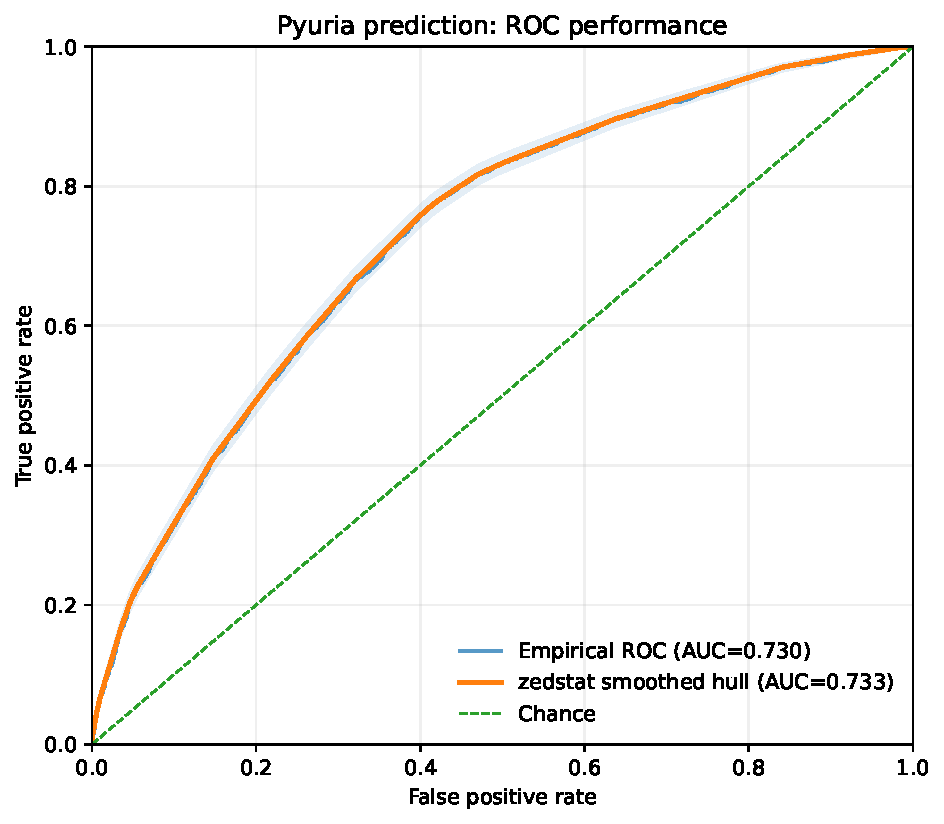
\includegraphics[width=.47\textwidth]{figures/roc_curve_zedstat.pdf}\hfill
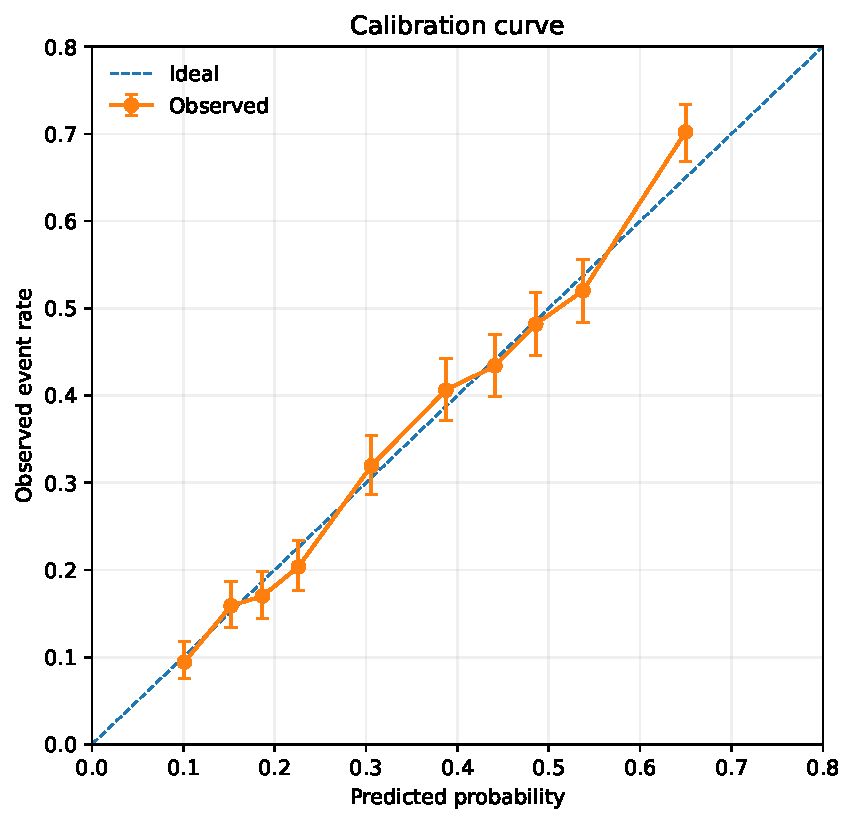
\includegraphics[width=.47\textwidth]{figures/calibration_curve_zedstat.pdf}
\end{center}

\newpage
\noindent\textbf{Calibration.} Brier score is 0.1934 (95\% CI 0.1894--0.1974). Calibration intercept is 0.0426 (95\% CI -0.0197--0.1053) and slope is 1.064 (95\% CI 0.999--1.134), both compatible with the ideal values 0 and 1. The highest risk decile shows mild underprediction (mean predicted risk $\approx0.650$ vs observed event rate $\approx0.702$).

\vspace{5pt}
\noindent\textbf{High-specificity operating points.}
\begin{table}[h!]
\centering
\small
\begin{tabular}{lrrr}
\toprule
Specificity & Sensitivity & PPV & LR+ \\
\midrule
0.90 & 0.316 & 0.629 & 3.16 \\
0.95 & 0.213 & 0.696 & 4.27 \\
0.99 & 0.0668 & 0.782 & 6.68 \\
\bottomrule
\end{tabular}
\end{table}

\noindent\textbf{Most important predictors.} Held-out SHAP magnitude and LightGBM gain both identify age, gender, weight, prior pyuria history, prior urine-WBC state, CBC/inflammatory measurements, pre-UA laboratory burden, albumin, creatinine, pulse, and admission-to-UA timing as dominant contributors. The top held-out SHAP variables are:

\begin{table}[h!]
\centering
\small
\begin{tabular}{rlr}
\toprule
Rank & Feature & Mean $|$SHAP$|$ \\
\midrule
1 & AGE & 0.312 \\
2 & GENDER & 0.306 \\
3 & WT\_KG & 0.205 \\
4 & prior\_pyuria\_rate & 0.0947 \\
5 & lab\_neutrophil\_abs & 0.0894 \\
6 & prior\_ua\_wbc\_last & 0.0677 \\
7 & lab\_cbc\_wbc & 0.0636 \\
8 & preUA\_lab\_count & 0.0614 \\
9 & lab\_Albumin\_Plasma & 0.0564 \\
10 & lab\_creatinine & 0.0512 \\
\bottomrule
\end{tabular}
\end{table}

\begin{center}
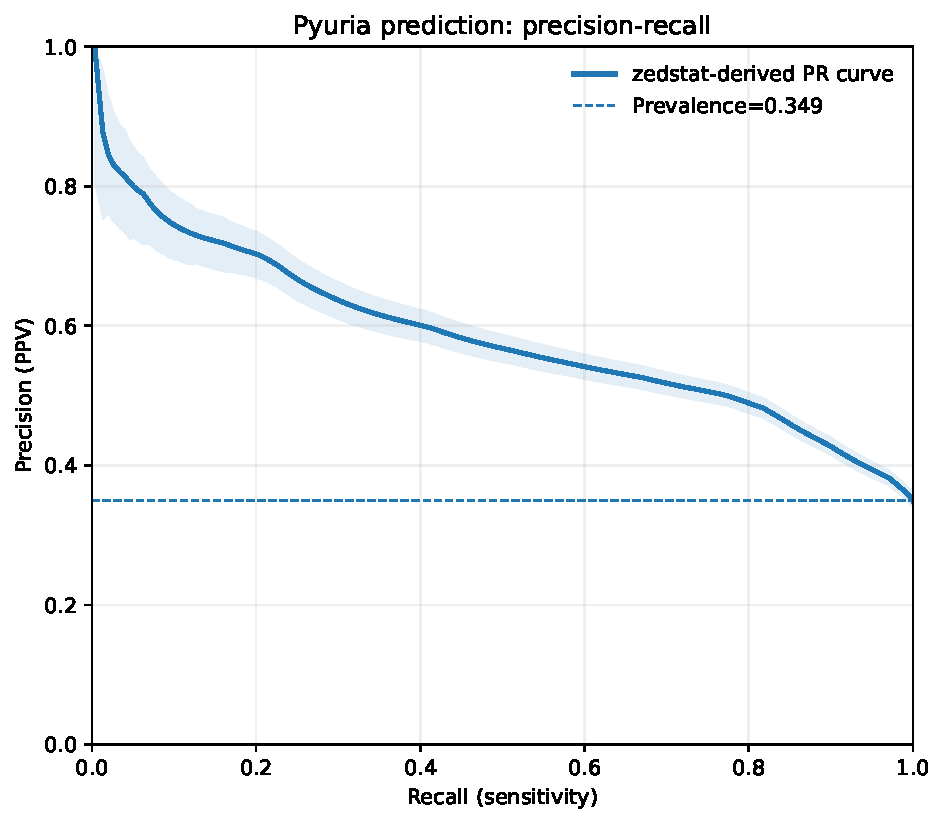
\includegraphics[width=.47\textwidth]{figures/precision_recall_zedstat.pdf}\hfill
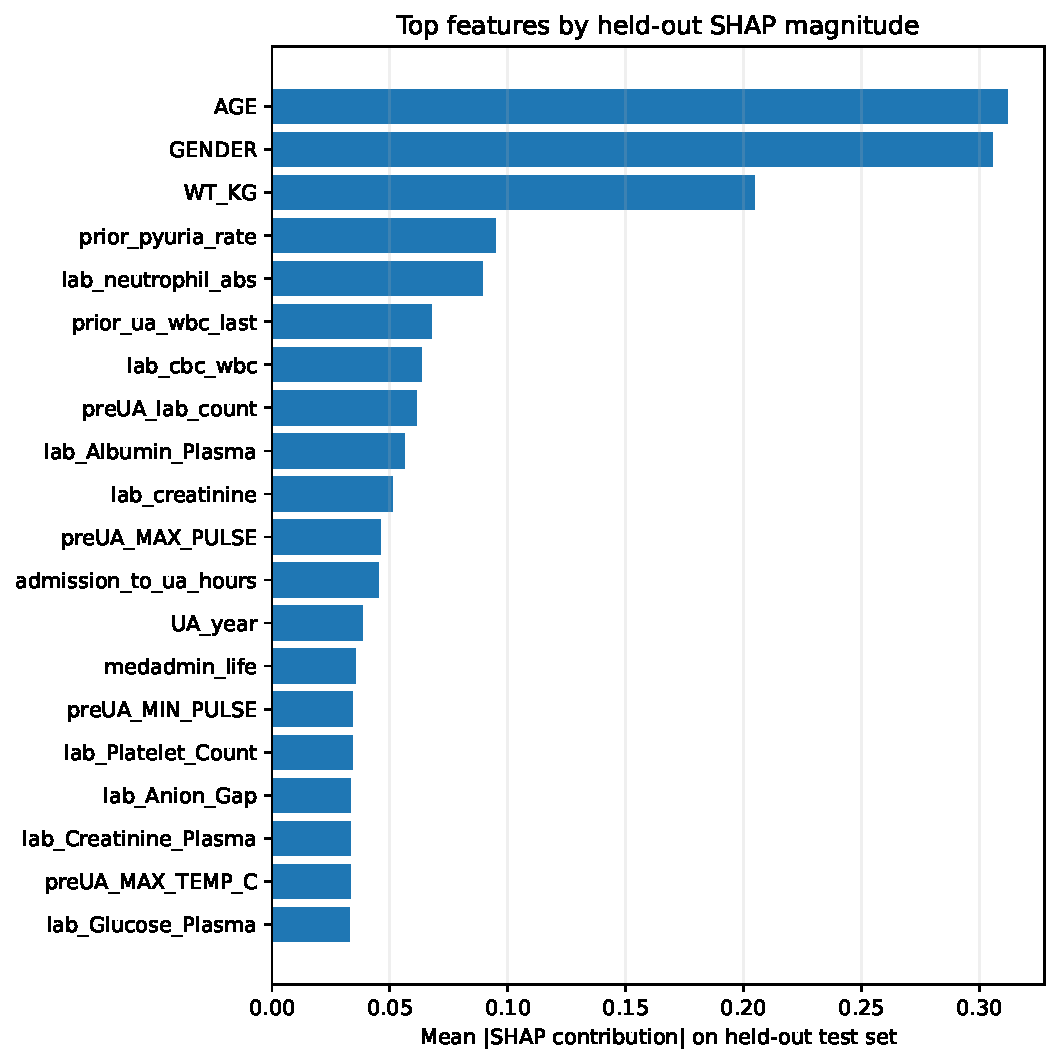
\includegraphics[width=.47\textwidth]{figures/feature_importance_shap.pdf}
\end{center}

\noindent\textbf{Interpretation.} Richer, carefully censored pre-UA EHR data produced the largest performance gain. Multiscale LSM conditionals add a smaller but consistent increment beyond LightGBM. The analysis is retrospective and should be externally validated before clinical use.

\vfill
\noindent\footnotesize Full methodology, all models, aggregate zedstat outputs, and reproducibility scripts are in this repository. No patient-level data are versioned here.

\end{document}
